\chapter{Simplicial Complexes and Homology}
\graphicspath{ {/home/tomasp/Dokumenty/Master_Thesis/figures/} }
%% Definitions, notations, remarks and examples
\theoremstyle{definition}
\newtheorem{definition}{Definition}[section]
\newtheorem{theorem}{Theorem}[section]
\newtheorem{lemma}{Lemma}[section]
\newtheorem{corollary}{Corollary}[section]
\newtheorem{example}{Example}[section]
\newtheorem*{remark}{Remark}

The goal of this and the following chapters is to establish and set up the pipeline for extracting the algebraic invariants of our data. Usually, we can only work with sampled and discrete data coming from some set of measurements. As such, we can't directly use methods of algebraic topology, since we won't typically be working with discrete topological spaces and to properly use these methods, we would need an uncountable amount of data; something that isn't feasible from a computational point of view.
\par
This forces us to use different methods to somehow approximate and recover the topology of the ambient space given only a finite set of points. Secondly, we also need to consider the \textit{scale} of the data -- some interesting properties may be more apparent only after we ``zoom'' in closely on them, some may not become apparent at all. All in all, we will construct the following pipeline:

\begin{center}
  \smartdiagram[sequence diagram]{
    Discrete data, Simplicial complex, Algebraic invariants}
\end{center}

and repeat this step for all scales at once, effectively measuring the evolution of the algebraic invariants through the changes in the feature scale.

\section{Simplicial complexes}
\begin{definition}[Simplex]
  For $k \geq 0$, a $k$-simplex $\sigma$ of dimension $k$ in a Euclidean space $\mathbb{R}^{n}$ is the convex hull of a set $P$ of $(k+1)$ affinely independent points in $\mathbb{R}^{n}$. For $0 \leq m \leq k$, an $m$-face of $\sigma$ is an $m$-simplex that is the convex hull of a nonempty subset of $P$. A \textit{proper face} of $\sigma$ is a simplex that is the convex hull of a proper subset of $P$ (any face except $\sigma$). $(k-1)$ faces of $\sigma$ are called \textit{facets} of $\sigma$.
\end{definition}

Typically, we refer to a $0$-simplex as a \textit{vertex}, a $1$-simplex as an \textit{edge}, a $2$-simplex as a \textit{triangle} and so on. An illustration of those can be seen in \ref{fig:simplex_1}.

\begin{figure}[h!]
  \centering
  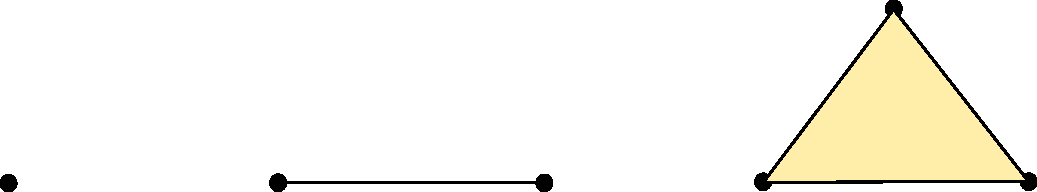
\includegraphics[width=10cm, height=2cm]{simplex_1.pdf}
  \caption{From the left: a $0$-simplex, a $1$-simplex and a $2$-simplex}
  \label{fig:simplex_1}
\end{figure}

\begin{definition}[Geometric simplicial complex]
  A \textit{geometric simplicial complex} $K$ is a set with finitely many simplices that satisfy the following:
  \begin{itemize}
  \item $K$ contains every face of each simplex in $K$.
  \item For any two simplices $\sigma, \tau \in K$, their intersection $\sigma \cap \tau$ is either empty or a face or both $\sigma$ and $\tau$.
  \end{itemize}
\end{definition}

This is also known as a \textit{triangulation}, where the \textit{dimension} $k$ of $K$ is the maximum dimension of any simplex in $K$. The two definitions above are highly geometric and easy to visualize and imagine. The next definition is more technical and abstract but nonetheless important.

\begin{definition}[Abstract simplex]
  A collection $K$ of non-empty subsets of a given set $V(K)$ is an \textit{abstract simplicial complex}, if every element $\sigma \in K$ has all of its non-empty subsets $\sigma' \subseteq \sigma$ also in $K$. Each element $\sigma$ with a cardinality $|\sigma| = k+1$ is called a $k$-simplex and each of its subsets $\sigma' \subseteq \sigma$ with $|\sigma'|=k'+1$ is called a $k'$-face. Finally, a $(k-1)$-face of a $k$-simplex is called its \textit{facet}.
\end{definition}

\begin{remark}
  One could also dually define a $k$-coface, cofacet and its codimension but it's not terribly important.
\end{remark}

\begin{figure}[h!]
  \centering
  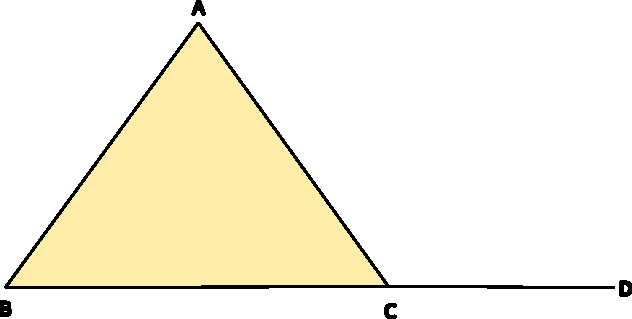
\includegraphics[width=8cm, height=4cm]{simplex_2.pdf}
  \caption{A simplicial complex with 4 vertices, 4 edges and 1 triangle.}
  \label{fig:simplex_2}
\end{figure}

A geometric simplicial complex $K$ in $\mathbb{R}^{n}$ is called a \textit{geometric realization} of an abstract simplicial complex $K'$, if and only if there is an embedding $e: V(K') \to \mathbb{R}^{n}$, that takes every $k$-simplex $\{v_{0}, \ldots, v_{k}\}$ in $K'$ to a $k$-simplex in $K$ that is the convex hull of $e(v_{0}), \ldots, e(v_{k})$. An example is shown in \ref{fig:simplex_2} as this is the geometric realization of the abstract complex with vertices $A,B,C,D,$ edges $\{A,B\}, \{A,C\}$,
$\{B,C\}, \{C,D\}$ and 1 triangle $\{A,B,C\}$.

\begin{definition}[Underlying space]
  The \textit{underlying space} of an abstract simplicial complex $K$, denoted by $|K|$, is the pointwise union of its simplices in its geometrical realization, i.e., $|K| = \bigcup_{\sigma \in K}|\sigma|$, where $|\sigma|$ is the restriction of this realization on $\sigma$. If $K$ is geometric, then its geometric realization can be taken as itself.
\end{definition}

Unless it is considered necessary, we won't be making the distinction between the two due to this equivalence between geometric and abstract simplicial complexes.

\begin{definition}[$k$-skeleton]
  For any $k \geq 0$, the $k$-skeleton of a simplicial $K$ complex, denoted by $K^{k}$, is the subcomplex formed by all simplices of dimension at most $k$.
\end{definition}
Given this, in \ref{fig:simplex_2}, the $1$-skeleton consists of the vertices $A,B,C,D$ and the edges joining those.

\section{Nerves, Čech and Rips complexes}
Given any open cover of a topological space, we are able to construct a simplicial complex on top of it. As we'll see, there isn't only one kind of complex we can build, depending on the properties we're looking for and its size, which has to be considered whenever we talk about any software implementation of the algorithms.

\begin{definition}[Nerve]
  Given a finite collection of sets $\mathfrak{U} = \{U_{\alpha}\}_{\alpha \in A}$, we define the \textit{nerve} of the set $\mathfrak{U}$ to be the simplicial complex $N(\mathfrak{U})$, whose vertex set is the index set $A$, and where a subset $\{\alpha_{0}, \ldots, \alpha_{k}\} \subseteq A$ spans a $k$-simplex in $N(\mathfrak{U})$ if and only if $U_{\alpha_{0}} \cap \ldots \cap U_{\alpha_{k}} \ne \emptyset$.
\end{definition}

\begin{figure}[h!]
  \centering
  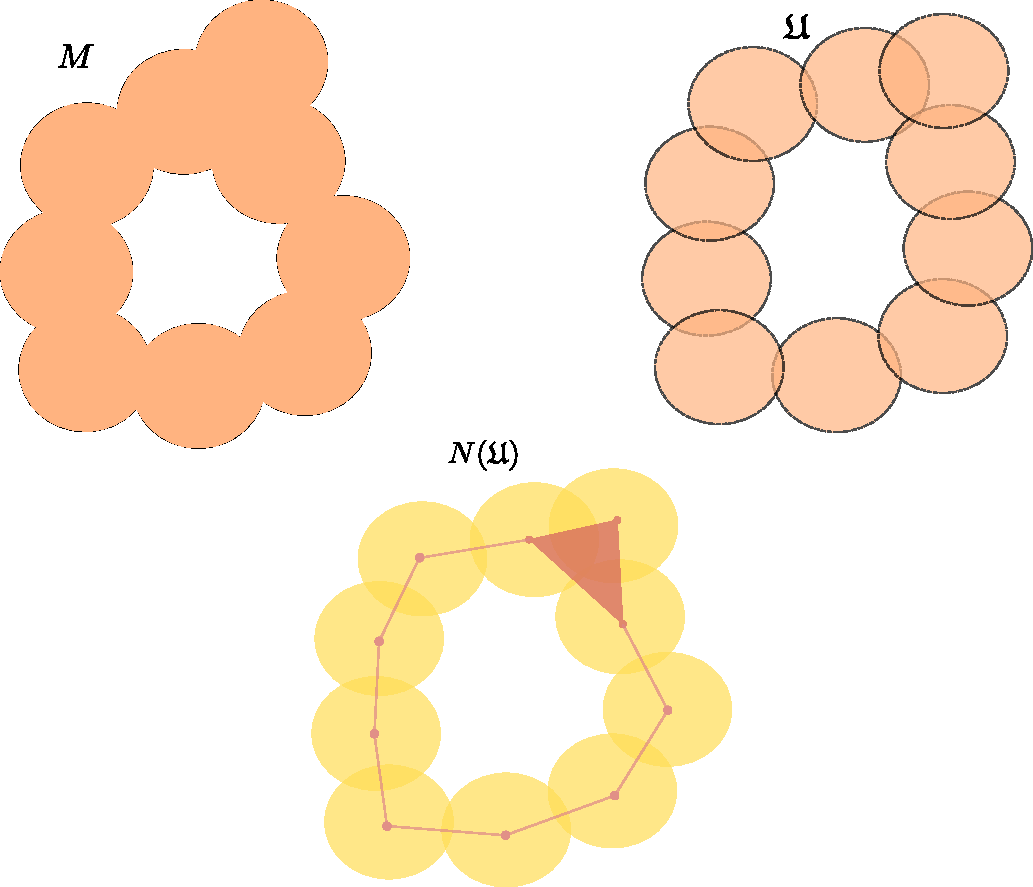
\includegraphics[width=10cm, height=8cm]{nerve_1.pdf}
  \caption{An example of a space $M$, its open cover $\mathfrak{U}$ and its nerve $N(\mathfrak{U})$.}
  \label{fig:nerve_1}
\end{figure}

The following important theorem about nerves tells us when are the nerves ``equivalent'' to the original space. There are various formulation of this statement but since we are working primarily with finite metric spaces, we'll adopt the appropriate version for it.

\begin{theorem}[Nerve theorem]
  Given a finite cover $\mathfrak{U}$ (open or closed) of a metric space $M$, the underlying space $|N(\mathfrak{U})|$ is homotopy equivalent to $M$, if every non-empty intersection $\cap_{i=0}^{k}U_{\alpha_{i}}$ of cover elements is homotopy equivalent to a point, i.e., contractible.
  \label{theorem:Nerve theorem}
\end{theorem}

For those interested in a proof of this statement, see \cite{Borsuk1948OnTI} for example. From this we can see, that the nerve is homotopy equivalent to $M$ in \ref{fig:nerve_1}. Now we can finally present the first construction of an abstract simplicial complex using the concept of a nerve, given a finite subset $P$ of a metric space $(M,d)$.

\begin{definition}[Čech complex]
  Let $(M,d)$ be a metric space and $P$ a finite subset of it. Given a real $\varepsilon > 0$, the Čech complex $\mathbb{C}^{\varepsilon}(P)$ is defined to be the nerve of the set $\{B(p_{i},\varepsilon)\}$, where
  \begin{equation*}
    B(p_{i},\varepsilon) = \{x \in M \: \vert \: d(p_{i},x) \leq \varepsilon \}.
  \end{equation*}
\end{definition}

One can easily deduce that if $M$ happens to be a Euclidean metric space, according to Theorem~\ref{theorem:Nerve theorem}, the Čech complex will be homotopy equivalent to the space of union of the balls. The Čech complex has nice theoretical properties, but the one predominantly implemented in most software packages is the Vietoris-Rips complex bellow.

\begin{definition}[Vietoris-Rips complex]
  Let $(P,d)$ be a finite metric space. Given a real $\varepsilon>0$, the Vietoris-Rips (VR for short) complex is the abstract simplicial complex $\mathbb{VR}^{\varepsilon}(P)$, where a simplex $\sigma \in \mathbb{VR}^{\varepsilon}(P)$, if and only if $d(p,q) \leq 2\varepsilon$ for every pair of vertices of $\sigma$.
\end{definition}

\begin{figure}[h!]
  \centering
  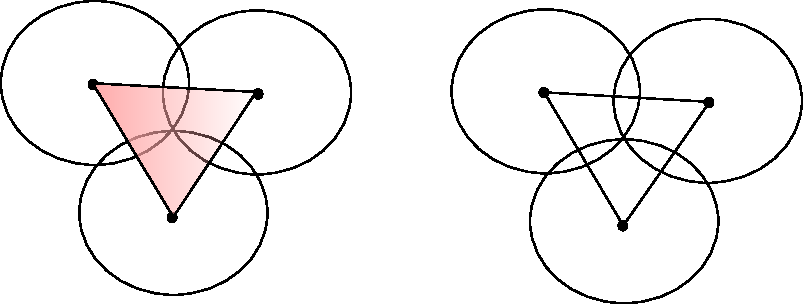
\includegraphics[width=8cm, height=4cm]{CechVR.pdf}
  \caption{On the left, the VR complex of three pairwise intersecting circles. On the right, the corresponding Čech complex.}
  \label{fig:CechVR}
\end{figure}

A simple example, where we can see the difference between the Čech and VR complex can be seen on \ref{fig:CechVR}. For an interactive visualization of the two, the reader may want to access the following sites - \cite{smajhiVietorisx2013RipsComplex} and \cite{saulnechComplex}. With the movement of the sliders there, the reader is introduced to another important concept that we will make use of - changing the radius $r$ and constructing a growing sequence of either Čech or VR complexes.

Nevertheless, we don't have to worry too much about the differences between the two, given the following result.

\begin{theorem}
  Let $P$ be a finite subset of a metric space $(M,d)$. Then
  \begin{equation}
    \mathbb{C}^{\varepsilon}(P) \subseteq \mathbb{V}^{\varepsilon}(P) \subseteq \mathbb{C}^{2\varepsilon}(P).
  \end{equation}
\end{theorem}

\section{Sparse complexes}

While the VR complex is the one you will usually encounter in most talks about TDA, it has a size problem. More often than not, both the Čech and VR complexes grow too large, even in low dimensions. A VR complex constructed out of a few thousand points can easily have millions of triangles. A short example of this behaviour can be seen in \ref{fig:sizeofVR}. As such, sometimes it is computationally less expensive to use more sparse alternatives instead. \footnote{Technically, the graph is based on the Rips filtration, a term we'll see in the future although it doesn't change the point presented here.}

\begin{figure}[h!]
  \centering
  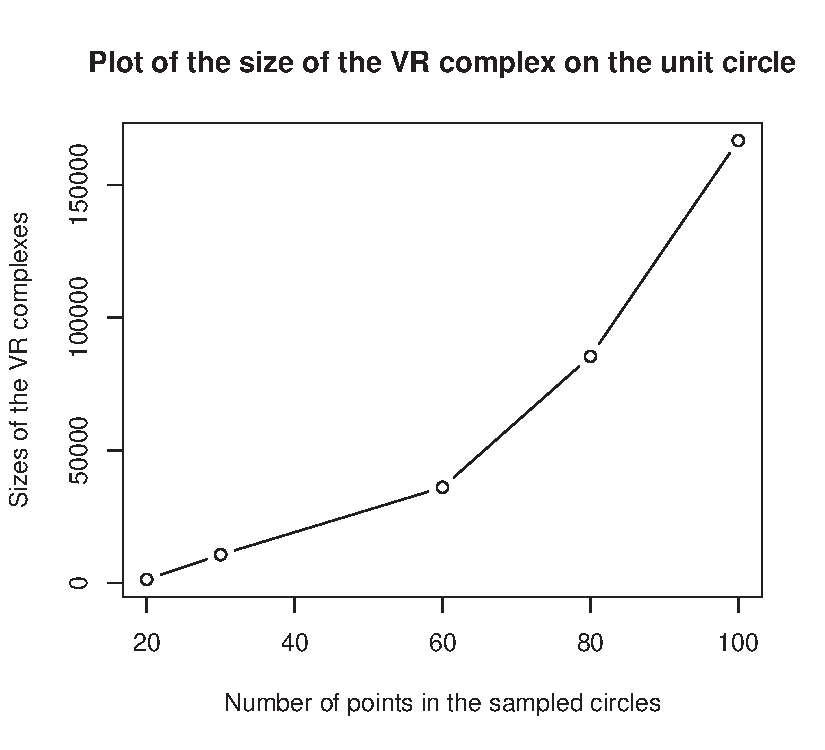
\includegraphics[width=8cm, height=8cm]{sizeofVR.pdf}
  \caption{An illustration of the growth of the VR complex when we increase the number of sampled points.}
  \label{fig:sizeofVR}
\end{figure}

\subsection{Delaunay complex}

This complex is usually used in various applications, such as mesh generation or 3D triangulation (for example, see \href{https://doc.cgal.org/latest/Manual/packages.html#PartTriangulationsAndDelaunayTriangulations}{the following}). However, it remains computationally expensive in dimensions greater than 3, and other complexes are preferred instead.

\begin{definition}[Delaunay complex]
  Let $P$ be a finite point set in $R^{n}$. A $k$-simplex $\sigma$ is called \textit{Delaunay}, if its vertices are in P and there is an open $n$-ball whose boundary contains the boundary of this ball. A \textit{Delaunay complex} of $P$, denoted by Del $P$, is the simplicial complex with vertices in $P$, in which every simplex is Delaunay and $\vert$ Del $P \vert$ coincides with the convex hull of $P$.
\end{definition}

\begin{figure}[h!]
  \centering
  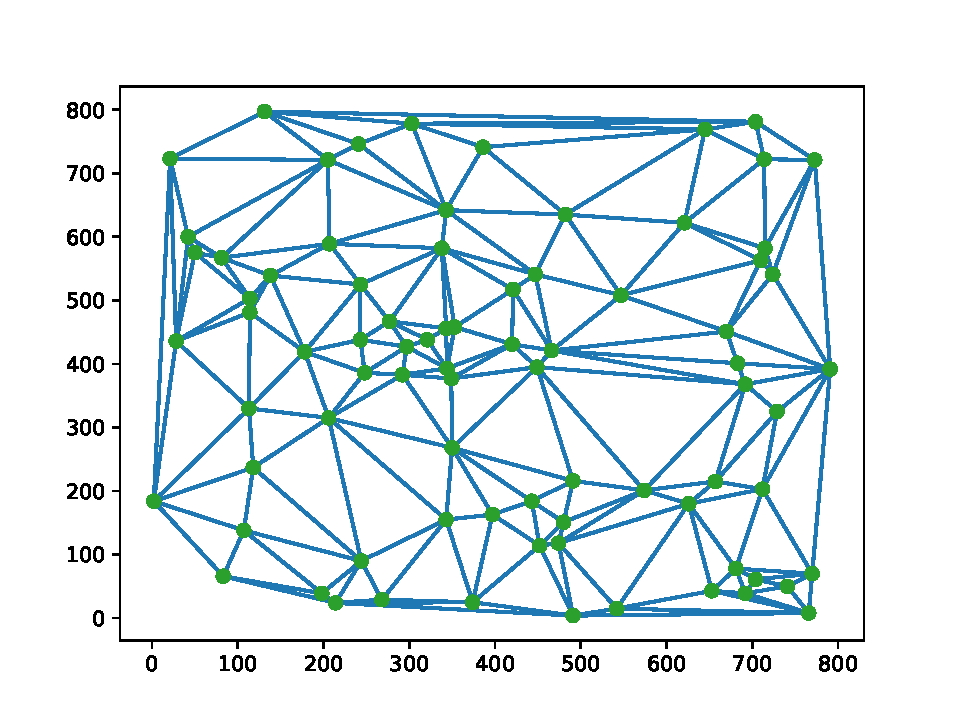
\includegraphics[width=10cm, height=8cm]{Delaunay.pdf}
  \caption{Delaunay complex on a sample of randomly generated points.}
  \label{fig:Delaunay}
\end{figure}

An example of a Delaunay complex can be seen on \ref{fig:Delaunay}. The Delaunay complex is dual to another construction that you may or may not encounter in the wild - the Voronoi diagram.

\begin{definition}[Voronoi diagram]
  Given a finite point set $P \subset \mathbb{R}^{n}$ in generic position, the Voronoi diagram Vor($P$) of $P$ is the tessellation of the embedding space $\mathbb{R}^{n}$ into convex cells $V_{p}$ for every $p \in P$ where
  \begin{equation*}
    V_{p} = \{x \in \mathbb{R}^{n} \: \vert \: d(x,p) \leq d(x,q), \forall q \in P\}.
  \end{equation*}
  Additionally, a $k$-face of Vor($P$) is the intersection of $(d-k+1)$ Voronoi cells.
\end{definition}

The duality between a Delaunay complex and Voronoi diagram is better expressed through this little theorem.
\begin{theorem}
  For $P \in \subset \mathbb{R}^{n}$, Del($P$) is the nerve of the set of Voronoi cells $\{V_{p}\}_{p \in P}$, which is a closed cover of $\mathbb{R}^{n}$.
\end{theorem}
More specifically, a Delaunay $k$-simplex in Del($P$) is dual to a Voronoi $(d-k)$-face in Vor($P$). That duality can be seen on \ref{fig:Voronoi}.
\footnote{Both \ref{fig:Delaunay} and \ref{fig:Voronoi} were generated using \cite{2020SciPy-NMeth}.}
The reasons why Delaunay complexes are popular in dimensions $<3$ are the following

\begin{figure}[h!]
  \centering
  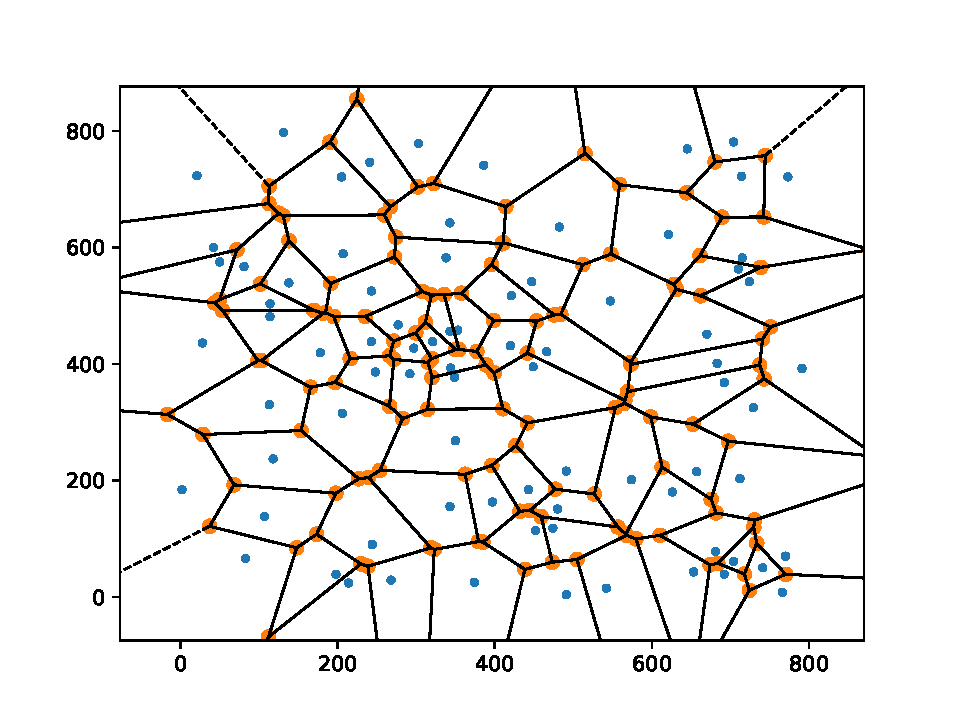
\includegraphics[width=10cm, height=8cm]{Voronoi.pdf}
  \caption{Voronoi diagram on a sample of randomly generated points dual to \ref{fig:Delaunay}.}
  \label{fig:Voronoi}
\end{figure}

\begin{theorem}
  A triangulation of a point set $P \subset \mathbb{R}^{n}$ is a geometric simplicial complex whose vertex set is $P$ and whose simplices tessellate the convex hull of $P$. Among all triangulations of a point set $P \subset \mathbb{R}^{n}$, Del($P$) achieves the following:
  \begin{enumerate}
  \item In $\mathbb{R}^{2}$, Del($P$) maximizes the minimum angle of triangles in the complex.
  \item In $\mathbb{R}^{2}$, Del($P$) minimizes the largest circumcircle for triangles in the complex.
  \item For a simplex in Del($P$), let its min-ball be the smallest ball that contains the simplex in it. In all dimensions, Del($P$) minimizes the largest min-ball.
  \end{enumerate}
\end{theorem}
Unfortunately, the size of a Delaunay complex is $O(n^{\lceil d/2 \rceil})$, with the same cost in computation (see \cite{chazelle1993optimal}).

\subsection{Alpha complex}
Alpha complexes are parametrized subcomplexes of the Delaunay complex by some real $\alpha \geq 0$. More specifically, for a given point set $P$ and some $\alpha \geq 0$, an alpha complex consists of all simplices in Del($P$) that have a circumscribing ball of radius at most $\alpha$. An alternative but equivalent definition follows like this - for each point $p \in P$, let $B(p,\alpha)$ be the closed ball of radius $\alpha$ centered at $p$. Consider the closed set $D^{\alpha}_{p}$ be defined as:
\begin{equation*}
  D^{\alpha}_{p} = \{x \in B(p,\alpha) \: \vert \: d(x,p) \leq d(x,q), \forall q \in P\}.
\end{equation*}
Then the alpha complex $\text{Del}^{\alpha}(P)$ is the nerve of the closed sets $\{D^{\alpha}_{p}\}_{p \in P}$.
We can use the duality of the Delaunay complex to introduce a third definition - an alpha complex contains a $k$-simplex $\sigma = \{p_{0}, \ldots, p_{k}\}$, if and only if $\bigcup_{p \in P}B(p,\alpha)$ meets the intersection of Voronoi cells $V_{p_{0}} \cup \ldots \cup V_{p_{k}}$.

\subsection{Graph induced complex}
Lastly, we present here another sparse complex that instead uses subsampling to tackle the size problem that the VR or Čech complexes have, while capturing the topology and even the geometry of the point cloud more efficiently. This construction was introduced in \cite{dey2013graphinducedcomplexpoint}.

\begin{definition}[Graph induced complex]
  Let $(P,d)$ be a metric space, where $P$ is a finite set and $G(P)$ be a graph with vertices in $P$. Let $Q \subseteq P$ and let $\nu : P \to Q$ the mapping that sets $\nu(p)$ to be any point in argmin $d(p,Q)$. The \textit{graph induced complex} (GIC) $\mathbb{G}(G(P),Q,d)$ is the simplicial complex containing a $k$-simplex $\sigma=\{q_{1}, \ldots, q_{k+1}\}$, $q_{i} \in Q$, if and only if there exists a $(k+1)$-clique in $G(P)$ spanned by vertices $\{p_{1}, \ldots, p_{k+1}\} \subseteq P$ so that $q_{i} \in \nu(p_{i})$ for each $i \in \{1,2, \ldots, k+1\}$.
\end{definition}

For the input graph $G(P)$ we may consider the neighborhood graph $G^{\alpha}(P) := (P,E)$, where there is an edge $\{p,q\} \in E$, if and only if $d(p,q) \leq \alpha$. If $P$ is sufficiently dense, then $G^{\alpha}(P)$ should capture the local neighborhoods of the sample points.

In the following, the quality of the sampled space after subsampling with $Q$ will be quantified with a parameter $\delta > 0$.

\begin{definition}
  A subset $Q \subseteq P$ is called a $\delta$-sample of a metric space $(P,d)$, if the following condition holds:
  \begin{itemize}
  \item $\forall p \in P$, there exists a $q \in Q$, so that $d(p,q) \leq \delta$.
  \end{itemize}
  It is called $\delta$-sparse, if the previous and next condition hold together:
  \begin{itemize}
  \item $\forall (q,r) \in Q \times Q$ with $q \neq r$, $d(q,r) \geq \delta$.
  \end{itemize}
\end{definition}
The metric itself is usually taken to be either the Euclidean metric or the graph metric $d_{G}$ derived from the input graph $G(P)$. In those two cases we have several existence and inference results involving the GIC; see \cite{dey2013graphinducedcomplexpoint} again for that. The paper also includes an empirical comparison of the GIC with the VR complex together with another sparse complex, the Witness complex, which we won't discuss in this thesis. The simulations show that the GIC can have a size similar to the Witness complex (which is usually smaller but also fails to capture the topology more because of it) and maintains the accuracy of the Rips complex.

\section{Chains, cycles and homology}
We make the daring assumption that the reader has some knowledge of algebra, group theory and topology in order to understand the next part. If not, maybe an appendix will be written in the future, who knows?

\subsection{Chains}
If $K$ is a simplicial $k$-complex with a $m_{p}$ number of $p$-simplices, then a $p$-chain $c$ in $K$ is simply the formal sum of $p$-simplices multiplied by some coefficients from a ring $R$. Addition of $p$-chains is defined in the following natural way: if $c = \sum \alpha_{i}\sigma_{i}$ and $c' = \sum \alpha_{i}'\sigma_{i},$ then

\begin{equation*}
  c + c' = \sum_{i=1}^{m_{p}} (\alpha_{i} + \alpha_{i}')\sigma_{i}.
\end{equation*}

Generally speaking, the multiplication by coefficients from $R$ turn chains into an $R$-module. In the context of this work, we will only consider coefficients coming from some field $\boldsymbol{k},$ more specifically from $\boldsymbol{k} = \mathbb{Z}_{2}$. This is computationally convenient because it turns chain addition into, for example in the case of 1-chains,

\begin{equation*}
  (e_{1} + e_{2} + e_{3}) + (e_{1} + e_{2} + e_{4}) = e_{3} + e_{4},
\end{equation*}

since in $\mathbb{Z}_{2}$ we have that $0 + 0 = 0, 0 + 1 = 1$ and $1+1 = 0$. This also implies that

\begin{equation*}
  c + c = \sum_{i=1}^{m_{p}} = (\alpha_{i} + \alpha_{i})\sigma_{i} = 0\sigma_{i} = 0,
\end{equation*}

i.e., $p$-chains with $\mathbb{Z}_{2}$ addition form a group, the identity here is the chain $0 = \sum_{i=1}^{m_{p}}0\sigma_{i}$, and the inverse of $c$ is $c$ itself due to the above. We call this group the \textit{$p$-th chain group} $C_{p}(K)$.

\subsection{Boundary operator and cycles}
Since our goal is to study the changes in topology across different scales, we need a way to connect higher dimensional chains with lower dimensional ones. For that, we introduce the boundary operator: Given a $p$-simplex $\sigma = \{v_{0}, \ldots, v_{p}\}$, let

\begin{equation*}
  \partial_{p}\sigma = \sum_{i=0}^{p}\{v_{0}, \ldots, \hat{v}_{i}, \ldots, v_{p}\},
\end{equation*}
where $\hat{v}_{i}$ means that this vertex is omitted. Extending this definition to a $p$-chain, we get the boundary operator homomorphism $\partial_{p}: C_{p} \to C_{p-1}$ that returns a $(p-1)$-chain when given a $p$-chain in the following manner

\begin{equation*}
  \partial_{p}c = \sum_{i=1}^{m_{p}}\alpha_{i}(\partial_{p}\sigma_{i}), \: \text{for} \: c = \sum_{i=1}^{m_{p}}\alpha_{i}\sigma_{i} \in C_{p}.
\end{equation*}

A couple edge cases have to be considered. For $p = 0$, we get that $\partial_{0}c = \emptyset$. The chain group $C_{-1}$ has only one element $0$. And if $K$ is a $k$-complex, then $C_{p} = 0$ for $p>k$. In general, most textbooks and articles will present the form of the boundary operator as follows:

\begin{equation*}
  \partial_{p}\sigma = \sum_{i=0}^{p}(-1)^{i} \{v_{0}, \ldots, \hat{v}_{i}, \ldots, v_{p}\},
\end{equation*}

which differs from our choice by the factor of $(-1)^{i}$. But remember that we're working in $\mathbb{Z}_{2}$, where the multiplicative factor becomes unnecessary due to the addition laws. As such, the boundary operator applied to the $2$-chain $\{a,b,c\}$ gives us

\begin{equation*}
  \partial_{2}(abc) = ab + bc + ca,
\end{equation*}
instead of $ab - bc + ca$ as you may encounter in other texts.

Applying the boundary operator twice in a row turns out to produce the empty chain.

\begin{lemma}
  For $p>0$ and any $p$-chain $c$, $\partial_{p-1}\circ\partial_{p}(c) = 0$.
\end{lemma}

\begin{proof}
  Trivial; can be found in any textbook about algebraic topology, for example \cite{hatcher2002algebraic}.
\end{proof}

By extending the boundary operator now to chain groups, we can construct a sequence called a \textit{chain complex}:

\begin{figure}[h]
  \begin{tikzcd}
    0 = C_{k+1} \arrow[r, "\partial_{k+1}"] & C_{k} \arrow[r, "\partial_{k}"] & \cdots \arrow[r] & \cdots \arrow[r] & C_{1} \arrow[r, "\partial_{1}"] & C_{0} \arrow[r, "\partial_{0}"] & C_{-1}=0.
  \end{tikzcd}
\end{figure}
It can be worthwhile to mention that for $p \geq -1$, each of the $C_{p}$ is a vector space.

\subsection{Cycle and boundary groups}
Just like with the chain groups, we can identify two other natural groups of interests - the \textit{cycle} and \textit{boundary} groups. We start by defining what a cycle is - a $p$-chain $c$ is a $p$-cycle if $\partial c = 0$, i.e., a chain with an empty boundary.

The $p$-cycles form the \textit{$p$-th cycle group} $Z_{p}$ with the same chain addition operation inherited from chain groups. From the above, we can see that ker $\partial_{p} = Z_{p}$.

We saw that after applying the boundary operator to the $2$-chain $\{a,b,c\}$, the result was

\begin{equation*}
  \partial_2(abc) = ab + bc + ca.
\end{equation*}
This $1$-chain is a $1$-cycle since
\begin{equation*}
  \partial_{1}(ab + bc + ca) = (a+b) + (b+c) + (c+a) = 0.
\end{equation*}

It's not difficult to conclude from this that the boundary of a $p$-chain is a $(p-1)$-cycle. This begs the question - which $(p-1)$-chains can be obtained this way? We call the set of all $(p-1)$-chains that are the result of an application of the boundary operator $\partial_{p}$ on $p$-chains the \textit{$(p-1)$-th boundary group} $B_{p-1} = \partial_{p}(C_{p})$. This is equivalent to saying that $B_{p-1} = \text{im} \: \partial_{p}$. It is left as an exercise for the reader to check that $\partial_{p-1}B_{p-1} = 0$ for all $p>0$, which implies that $B_{p-1} \subseteq Z_{p-1}$.

\begin{theorem}
  For a simplicial $k$-complex,
  \begin{itemize}
  \item $C_{0} = Z_{0}$ and $B_{k} = 0$.
  \item For $p \geq 0$, $B_{p} \subseteq Z_{p} \subseteq C_{p}$.
  \item Both $B_{p}$ and $Z_{p}$ are vector spaces.
  \end{itemize}
\end{theorem}

\subsection{Homology}

We can finally define the most important notion in this work - homology. Homology is primarily used to quantify and measure the failure of a cycle to be a boundary by putting cycles that differ by a boundary in the same equivalence class.

\begin{definition}[Homology group]
  For $p \geq 0$, the \textit{$p$-th homology group} is the quotient group $H_{p} = Z_{p} / B_{p}$. Since we're using $\mathbb{Z}_{2}$ as our coefficient field, $H_{p}$ is a vector space, where we call its dimension the $p$-th Betti number
  \begin{equation*}
    \beta_{p} := \text{dim} \: H_{p}.
  \end{equation*}
\end{definition}

The equivalence classes are called \textit{homology classes} in this context. Two cycles $c, c' \in Z_{p}$ are in the same homology class, iff $c \in c' + B_{p}$, which under $\mathbb{Z}_{2}$ coefficients translates to $c + c' \in B_{p}$.

We have the following useful statements with our choice of field coefficients:

\begin{theorem}
  For $p \geq 0$,
  \begin{itemize}
  \item $H_{P}$ is a vector space when defined over $\mathbb{Z}_{2}$.
  \item The Betti number, $\beta_{p} = \text{dim}\:H_{p}$, is given by $\beta_{p} = \text{dim}\:Z_{p} - \text{dim}\:B_{p}$.
  \item There are exactly $2^{\beta_{p}}$ homology classes in $H_{p}$ when defined over $\mathbb{Z}_{2}$.
  \end{itemize}
\end{theorem}

Generally speaking, $H_{p}$ isn't always a vector space over $\mathbb{Z}$ as there might be torsion subgroups.

Now what is homology useful for, in the context of statistics and data analysis? The homology group $H_{n}(X)$ of some topological space, more specifically its Betti number, tells us the number of ``holes'' with a $n$-dimensional boundary in our data. For example, a $0$-dimensional hole is merely the gap between any two components. It implies then that $H_{0}(X)$ desribes the path-connected components in $X$. This turns out to be an strong, invariant characteristic of the dataset that we work with and allows us to discover high-dimensional structures that normally we wouldn't be able to notice.

A few informal examples may be useful to the reader; the proofs of which use more complicated techniques such as the Mayer-Vietoris sequence and so they will be omitted since this isn't an algebraic topology textbook. It isn't hard to see that $S^{1}$, the one-dimensional sphere, has only 1 path-connected component and 1 one-dimensional hole in the middle. We can then describe its homology groups as

\begin{equation*}
  H_{k}(S^{1}) = \begin{cases}
    \mathbb{Z} \qquad k = 0,1 \\
    \{0\} \quad \text{otherwise}
  \end{cases}
\end{equation*}

The corresponding Betti numbers here would be $\beta_{0} = \beta_{1} = 1$ and $\beta_{k} = 0, \forall k > 1$. This aligns with our intuition that a circle has a hole in the middle, one boundary line trapping said hole and no other high-dimensional structure. The argument can be extended for the general $n$-sphere to produce

\begin{equation*}
  H_{k}(S^{n}) = \begin{cases}
    \mathbb{Z} \qquad k = 0,n \\
    \{0\} \quad \text{otherwise}
  \end{cases}
\end{equation*}

With a little more effort and imagination, it isn't hard to see that the homology groups for the $2$-dimensional torus $T^{2}$ are

\begin{equation*}
  H_{k}(T^{2}) = \begin{cases}
    \mathbb{Z} \qquad \qquad k = 0,2 \\
    \mathbb{Z} \times \mathbb{Z} \qquad k = 1 \\
    \{0\} \qquad \text{otherwise}
  \end{cases}
\end{equation*}

where the two 1-dimensional holes describe the circles around the width and length of the torus. Once again, in general the situation is

\begin{equation*}
  H_{k}(T^{n}) = \begin{cases}
    \mathbb{Z}^{\binom{n}{k}} \qquad 0 \leq k \leq n  \\
    \{0\} \qquad \text{otherwise}
  \end{cases}
\end{equation*}

\subsection{Induced homology}
To have a better understanding of homology, we have to know how it behaves if we move from one topological space to another. In our case, we will look into simplicial complexes and simplicial maps between them since we can only ever approximate a continuous space. Simplicial maps take cycles to cycles and boundaries to boundaries, which suggests the following definition.

\begin{definition}[Chain map]
  Let $f:K_{1} \to K_{2}$ be a simplicial map. The chain map $f_{\#}: C_{p}(K_{1}) \to C_{p}(K_{2})$ corresponding to $f$ is defined as follows. If $c = \sum \alpha_{i}\sigma_{i}$ is a $p$-chain, then $f_{\#}(c) = \sum \alpha_{i} \tau_{i}$, where
  \begin{equation*}
    \tau_{i} =
    \begin{cases}
      f(\sigma_{i}), \quad \text{if} \: f(\sigma_{i}) \: \text{is a $p$-simplex in} \: K_{2} \\
      0 \qquad \quad \text{otherwise}.
    \end{cases}
  \end{equation*}
\end{definition}

\begin{lemma}
  Let $f: K_{1} \to K_{2}$ a simplicial map. Let $\partial_{p}^{K_{1}}$ and $\partial_{p}^{K_{2}}$ denote the boundary homomorphisms in dimension $p \geq 0$. Then, the induced chain maps commute with the boundary homomorphisms, i.e., $f_{\#} \circ \partial_{p}^{K_{1}} = \partial_{p}^{K_{2}} \circ f_{\#}$.
\end{lemma}

This result can be better expressed via the commutativity of the diagram below:

\begin{figure}[h]
  \centering
  \begin{tikzcd}
    C_{p}(K_{1}) \arrow[rr, "f_{\#}"] \arrow[dd, "\partial_{p}^{K_{1}}"] &  & C_{p}(K_{2}) \arrow[dd, "\partial_{p}^{K_{2}}"] \\
    &  &                                                 \\
    C_{p-1}(K_{1}) \arrow[rr, "f_{\#}"']                                 &  & C_{p-1}(K_{2})
  \end{tikzcd}
\end{figure}

Essentially, if we start from the top left, the path that we choose doesn't matter because we'll reach the same chain in the end. From the above, since $B_{p}(K_{1}) \subseteq Z_{p}(K_{1})$, we see that $f_{\#}(B_{p}(K_{1})) \subseteq f_{\#}(Z_{p}(K_{1}))$, which allows us to have a well defined induced map in the quotient space

\begin{equation*}
  f_{*}(Z_{p}(K_{1})/B_{p}(K_{1})) := f_{\#}(Z_{p}(K_{1})) / f_{\#}(B_{p}(K_{1})).
\end{equation*}

From the commutativity of the diagram, $f_{\#}(Z_{p}(K_{1})) \subseteq Z_{p}(K_{2})$, likewise for $B_{p}(K_{1})$, which then induces a homomorphism between the homology groups

\begin{equation*}
  f_{*}: Z_{p}(K_{1})/B_{p}(K_{1}) \to Z_{p}(K_{2})/B_{p}(K_{2}),
\end{equation*}
or $f_{*}: H_{p}(K_{1}) \to H_{p}(K_{2})$. We can now state the desired result.

\begin{lemma}
  For two contiguous maps $f_{1}: K_{1} \to K_{2}$ and $f_{2}: K_{1} \to K_{2}$, the induced maps $f_{1_{*}}: H_{p}(K_{1}) \to H_{p}(K_{2})$ and $f_{2_{*}}: H_{p}(K_{1}) \to H_{p}(K_{2})$ are equal.
\end{lemma}

\subsection{Cohomology}
Cohomology is the dual concept of homology. While in general cohomology has a richer structure and is a finer invariant than homology, in our case we won't explore the differences between the two as most of the popular software uses homology for their calculations. As usual, we will work with coefficients in $\mathbb{Z}_{2}$.

A $p$-cochain is a homomorphism $\phi: C_{p} \to \mathbb{Z}_{2}$ from the chain group to the coefficient ring $\mathbb{Z}_{2}$. The cochain is determined by its values on every $p$-simplex $\sigma \in K$, i.e., a $p$-chain $c = \sum_{i=1}^{m_{p}}\alpha_{i}\sigma_{i}$ assigns a value

\begin{equation*}
  \phi(c) = \alpha_{1}\phi(\sigma_{1}) + \ldots + \alpha_{m_{p}}\phi(\sigma_{m_{p}})
\end{equation*}

that is either $0$ or $1$. It isn't hard to verify that $\phi(c + c') = \phi(c) + \phi(c')$. The cochain that gives the value $1$ to a simplex is called its dual cochain $c^{*}$. $p$-cochains form the cochain group $C^{p}$ dual to $C_{p}$ with addition defined by $(\phi + \phi')(c) = \phi(c) + \phi'(c)$ and scalar multiplication $(\alpha \phi)(c) = \alpha \phi(c)$, where we used $\mathbb{Z}_{2}$ addition and multiplication. Hence, $C^{p}$ is a vector space.

Similarly to chain boundaries, there is the notion of a cochain coboundary $\delta_{p}: C^{p} \to C^{p+1}$. For a $p$-cochain $\phi$, its $(p+1)$-coboundary is given by the homomorphism $\delta \phi: C^{p+1} \to \mathbb{Z}_{2}$ defined as $\delta \phi(c) = \phi(\partial c)$ for any $(p+1)$-chain $c$. Repeated iteration of the $\delta$ operator gives us the sequence

\begin{figure}[h]
  \centering
  \begin{tikzcd}
    0 = C^{-1} \arrow[r, "\delta_{-1}"] & C^{0} \arrow[r, "\delta_{0}"] & \ldots \arrow[r, "\delta_{k-1}"] & C^{k} \arrow[r, "\delta_{k}"] & C^{k+1} = 0.
  \end{tikzcd}
\end{figure}

$p$-coboundaries form the coboundary group and vector space $B^{p}$ with addition and scalar multiplication being the same as in $C^{p}$. Finally, we only need cocycles to define what the cohomology group is. A $p$-cochain $\phi$ is called a $p$-cocycle if its coboundary $\delta \phi$ is a zero homomorphism. The set of $p$-cocycles forms the group and vector space $Z^{p}$ with the operations induced by $C^{p}$ once again.

The coboundary operator $\delta$ also satisfies the same property as the boundary $\partial$.

\begin{lemma}
  For $p >0$, $\delta_{p} \circ \delta_{p-1} = 0$, which implies $B^{p} \subseteq Z^{p}$.
\end{lemma}

\begin{definition}[Cohomology group]
  Since $B^{p}$ is a subgroup of $Z^{p}$, the $p$-th cohomology group is the quotient group $Z^{p} / B^{p}$.
\end{definition}

Just like for the homology groups, a simplicial map $f: K_{1} \to K_{2}$ induces a homomorphism $f^{*}$ between cohomology groups; this time in the \textit{opposite} direction.

\begin{lemma}
  A simplicial map $f: K_{1} \to K_{2}$ induces a homomorphism $f^{*}: H^{p}(K_{2}) \to H^{p}(K_{1})$ for every $p \geq 0$.
\end{lemma}

\section{Practical questions}

Now that we have a basic rundown of what simplicial complexes and homology are, we can move towards more practical questions. How do we actually compute the homology of an object? What is the available software? And the most important question, since we always have to work with discrete samples from some given space - can we accurately approximate the homology of a space given enough sample points?

\subsection{Calculating homology}

We can start by constructing a simplicial complex homeomorphic to the $2-$sphere $S^{2}$ as follows

\begin{figure}[h]
  \centering
  \begin{tikzcd}
    y \arrow[rrrr, "b"]                                                           &  &  &  & z                  \\
    &  &  &  &                    \\
    x \arrow[rrrr, "a"'] \arrow[rrrruu, "B"] \arrow[uu, "a"] \arrow[rrrruu, "A"'] &  &  &  & y \arrow[uu, "b"']
  \end{tikzcd}
\end{figure}

In this relatively simple example, its chain complex is characterized by

\begin{figure}[h]
  \centering
  \begin{tikzcd}
    \cdots \arrow[r] & 0 \arrow[r, "\partial_{3}"] & {\langle A,B \rangle} \arrow[r, "\partial_{2}"] & {\langle a,b,c \rangle} \arrow[r, "\partial_{1}"] & {\langle x,y,z \rangle} \arrow[r, "\partial_{0}"] & 0
  \end{tikzcd}
\end{figure}

Our goal will be to compure the homology group $H_{0}$ of this simplicial complex, and by extension, of $S^{2}$. We already know that $\text{ker}\:\partial_{0}\langle x,y,z \rangle$ is $\langle x,y,z \rangle$ itself. Now we need to figure out what $\text{Im}\:\partial_{1}$ is. For that, the behaviour of $\partial_{1}$ on any $1-$chain $la + mb + nc$ is needed.

Following the properties of the maps $\partial_{i}$, we have that

\begin{align*}
  \partial_{1}(la + mb + nc) &= l\partial_{1}(a) + m\partial_{1}(b) + n\partial_{1}(c) \\
  &= l(y-x) + m(z-y) + n(z-x) \\
  &= (-l-n)x + (l-m)y + (m+n)z.
\end{align*}

We can represent this chain with a $3-$tuple $[l,m,n]^{T} \in \mathbb{Z}^{3}$ since this is a finitely generated abelian group of rank $3$. Writing the equation above as a tranformation

\begin{equation*}
  [l,m,n]^{T} \to [-l-n,l-m,m+n]^{T},
\end{equation*}

allows us to represent the effect of $\partial_{1}$ as a matrix

\begin{equation*}
  [\partial_{1}] =
  \begin{pmatrix}
    -1 & 0 & -1 \\
    1 & -1 & 0 \\
    0 & 1 & 1
  \end{pmatrix}
\end{equation*}

Elementary row-reduction methods yield

\begin{equation*}
  \begin{pmatrix}
    1 & 0 & 1 \\
    0 & 1 & 1 \\
    0 & 0 & 0
  \end{pmatrix}
\end{equation*}

From this matrix, we can easily find a basis of $\text{Im}\:\partial_{1}$
\begin{equation*}
  [-1,1,0]^{T}, [0, -1, 1]^{T},
\end{equation*}
which corresponds to $(y-x)$ and $(z-y)$. Computing $H_{0}$ now amounts to computing the quotient
\begin{equation*}
  H_{0} = \langle x,y,z \rangle / \langle y-x, z-y \rangle.
\end{equation*}

We can identify $(y-x)$ and $(z-y)$, which forces the quotient homomorphism $q: \text{Ker}\:\partial_{1} \to H_{0}$ to behave as follows:
\begin{align*}
  q(y-x) &= q(y) - q(x) = 0 \Longrightarrow q(y) = q(x) \\
  q(z-y) &= q(z) - q(y) = 0 \Longrightarrow q(z) = q(y)
\end{align*}

To obtain the quotient, we first swap $y$ by $x$:
\begin{equation*}
  H_{0} = \langle x,x,z \rangle / \langle 0, z-x \rangle = \langle x,z \rangle / \langle z-x \rangle
\end{equation*}

Then we swap $z$ with $y$:
\begin{equation*}
  H_{0} = \langle x,x \rangle / 0 = \langle x \rangle
\end{equation*}

Therefore $H_{0} \cong Z$ and the $2-$sphere $S^{2}$ has only one connected component - itself. The essence of this example lies in reducing the calculation of homology groups to matrix manipulations. Typically, a homology solver will make use of the Smith normal form of a matrix.

\begin{definition}[Smith normal form]
  For any $m \times n$ matrix $A$, there exists an invertible $n \times n$ matrix $U$ and an invertible $m \times m$ matrix $V$ such that $UAV$ is equal to a matrix of the form
  \begin{equation*}
    D =
    \begin{bmatrix}
      \alpha_1 & 0 & 0 & & \dots & 0\\
      0 & \alpha_2 & 0 & & & 0\\
      0 & 0 & \ddots \\
      \vdots & & & \alpha_r \\
      & & & & 0\\
      0 & & & & & \ddots \\
      & & & & & & 0
    \end{bmatrix}
  \end{equation*}

  Furthemore, if $A$ is an integer matrix, then $U,V,D$ are all integer matrices and the $\alpha_{i}$ satisfy $\alpha_{i} | \alpha_{i+1}$ for all $1 \leq i < r$.
\end{definition}

For the computation of the homology groups, we use the following theorem that we won't prove here.

\begin{theorem}
  Let $A$ be a $m \times n$ integer matrix, $B$ an $l \times m$ integer matrix such that $BA = 0$. Then
  \begin{equation*}
    Ker(B)/Im(A) = \bigoplus_{i=1}^r \mathbb{Z}/\alpha_i \oplus \mathbb{Z}^{m-r-s},
  \end{equation*}
  where $r = rank(A), s = rank(B)$ and $\alpha_{1}, \ldots, \alpha_{r}$ are the non-zero elements on the diagonal of the Smith normal form of $A$.
\end{theorem}

Most homology solvers make use of additional optimization steps before resorting to matrix algebra. Libraries such as Linbox \cite{linbox} (written in C++) can be used to compute the Smith normal form. The library Perseus \cite{perseus} (written in C++) computes both ``standard'' and persistent homology, which we will discuss in later chapters. Kenzo \cite{kenzo} (written in Common Lisp) can additionaly give presentations of homology groups, implementing methods of so-called \textit{Constructive Algebraic Topology}. Gmsh \cite{gmsh} provides homology solvers for finite element meshes. There are many more open-source libraries in the wild, some of which we'll use in our applied examples.

But what about the stability and precision of this process? In the example we presented, there wasn't anything to worry about. On the other hand, what we will usually end up working with are simplicial complexes generated from sample data; the Čech and Vietoris-Rips complex, for example. Not only do we have to deal with errors of measurements and noise in our data but also the failure of our generated complex to match the ``true'' topological space where our data lives. The more precise formulation of this problem can be stated as: Let $(P, d)$ be a finite metric space of samples from a topological space $A$. When is $|\mathbb{VR}^{\varepsilon}(P, d)|$ or $|\mathbb{C}^{\varepsilon}(P, d)|$ homotopy equivalent to $A$?

We will attack the idea of \textit{geometric sampling} in later chapters as well, specifically, when we will introduce the idea of statistical testing and estimation while working with homology groups. For now, we can settle on a basic, minimal guarantee result known as the \textit{Niyogi-Smale-Weinberger theorem}. The idea of the theorem is that if we have sufficiently many points sample uniformly from a compact Riemannian manifold $M \subset \mathbb{R}^{n}$, there exists an isomorphism

\begin{equation*}
  H_{*}\left(\bigcup_{x \in M} B_{\varepsilon}(x) \right) \cong H_{*}(M)
\end{equation*}

with high probability for a suitable choice of $\varepsilon$. For a manifold $M \subset \mathbb{R}^{n}$, the choice of $\varepsilon$ is influenced by two factors -- its intrinsic curvature and how twisted the embedding into $\mathbb{R}^{n}$ is. The quantity used to encode the appropriate interval of $\varepsilon$ values is called the \textit{condition number}. The condition number is more precisely defined as the minimum radius at which the tubular neighbourhood of a manifold self-intersects.

\begin{theorem}[Niyogi-Smale-Weinberger theorem]
  Let $M$ be a compact submanifold of $\mathbb{R}^{n}$ with condition number $\tau$ and let $\{x_{1}, \ldots, x_{k}\}$ be a set of points drawn from $M$ according to the volume measure. Fix $0 < \varepsilon < \tau/2$. Then if
  \begin{equation*}
    k > \beta_{1}\left(\log(\beta_{2}) + \log(1/\delta) \right),
  \end{equation*}
  there is a homotopy equivalence
  \begin{equation*}
    \left(\bigcup_{z \in \{x_{1}, \ldots, x_{k}\}} B_{\varepsilon}(z) \right) \cong M
  \end{equation*}
  between the union of balls and $M$ with probability $> 1 - \delta$ and the homology groups coincide. Here
  \begin{equation*}
    \beta_{1} = \frac{\text{vol}\:(M)}{\cos^{n}(\theta_{1})\text{vol}\:(B^{n}_{\varepsilon/4})}
  \end{equation*}
  and
  \begin{equation*}
    \beta_{2} = \frac{\text{vol}\:(M)}{\cos^{n}(\theta_{2})\text{vol}\:(B^{n}_{\varepsilon/8})}
  \end{equation*}
  where $\theta_{1} = \arcsin(\frac{\varepsilon}{8\tau}), \theta_{2} = \arcsin(\frac{\varepsilon}{16\tau})$ and $\text{vol}\:(B^{n}_{r})$
  denotes the volume of the $n-$dimensional ball of radius $r$.
\end{theorem}

For example, the condition number of a sphere is its radius. For the unit $1-$sphere $S^{1} \subset \mathbb{R}^{2}$, $\delta = 0.01$ and $\varepsilon = \frac{1}{4}$, we obtain
\begin{equation*}
  \beta_{1} = 512, \quad \beta_{2} = 2048,
\end{equation*}
meaning that the minimum number of sample required is
\begin{equation*}
  512(7.6 + 4.6) \sim 6260.
\end{equation*}

While the result is theoretically important, its practical use is limited. The estimation of the condition number is usually difficult or simply impossible, and the obtained bound is too large, as the above example demonstrates. As such, we will rely on other methods and results that are computationally feasible while lowering the number of samples needed.
